\documentclass[8pt, landscape, a4paper]{extarticle}

% --- 核心宏包 ---
\usepackage[UTF8]{ctex}
\usepackage[margin=0.8cm, top=1cm, bottom=1.3cm]{geometry}
\usepackage{multicol}
\usepackage{xcolor}
\usepackage{tcolorbox}
\usepackage{enumitem}
\usepackage{amsmath}
\usepackage{amssymb}
\usepackage{fontspec}
\usepackage{tikz} % 【新增】用于画图

% --- 去掉页码 ---
\pagestyle{empty}

% --- 颜色定义 ---
\definecolor{headerblue}{RGB}{41, 128, 185}
\definecolor{section1}{RGB}{22, 160, 133} 
\definecolor{section2}{RGB}{41, 128, 185} 
\definecolor{section3}{RGB}{142, 68, 173} 
\definecolor{section4}{RGB}{211, 84, 0}   
\definecolor{section5}{RGB}{192, 57, 43}  
\definecolor{dividergray}{RGB}{220, 220, 220}

% --- 全局设置 ---
\setlength{\parindent}{0pt}
\setlength{\columnsep}{0.4cm} 
\linespread{1.1} 

% --- 列表样式 ---
\setlist[itemize]{leftmargin=1.2em, nosep, itemsep=2pt, topsep=2pt, label=$\vcenter{\hbox{\tiny$\bullet$}}$}
\setlist[description]{leftmargin=0.2em, style=sameline, nosep, itemsep=2pt, font=\bfseries}

% --- Box 样式 ---
\newtcolorbox{mybox}[2][]{%
  colback=white,
  colframe=#2,
  coltitle=white,
  boxrule=1pt,             
  arc=2mm,                 
  left=4pt, right=4pt, top=3pt, bottom=3pt, 
  toptitle=3pt, bottomtitle=3pt, 
  fonttitle=\bfseries\sffamily\large,
  title={#1},
  after skip=5pt          
}

% --- 自定义命令 ---
\newcommand{\subt}[1]{{\vspace{2pt}\textbf{\large \textcolor{black}{#1}}}}

\newcommand{\boxdesc}[1]{%
    \textit{\small \textcolor{gray}{#1}}%
    \par\vspace{2pt}%
    {\color{dividergray}\hrule height 0.5pt}%
    \vspace{2pt}%
}

\newcommand{\sepline}{%
    \par \vspace{3pt}%
    {\color{dividergray}\hrule height 0.5pt}%
    \par \vspace{3pt}%
}

% 公式间距设置
\setlength{\abovedisplayskip}{3pt}
\setlength{\belowdisplayskip}{3pt}

\begin{document}

% --- 页眉 ---
\begin{center}
    {\Huge \textbf{\sffamily 复变函数 Engineering Cheat Sheet}} \\
    \vspace{0.2cm}
    {\large \texttt{Complex Analysis: The Art of Rotation from Euler's Formula to Conformal Mapping}}
\end{center}

% --- 开始四栏布局 ---
\begin{multicols*}{4}

% === 第一栏 ===

\begin{mybox}[��️ 场景导航 (Use Cases)]{section4}
    \boxdesc{遇到什么问题 $\to$ 用什么工具}
    \begin{itemize}[itemsep=2pt]
        \item \textbf{处理震荡/周期} $\to$ 欧拉公式 (旋转)
        \item \textbf{解难算积分} $\to$ 留数定理 (数奇点)
        \item \textbf{不规则边界流体} $\to$ 保角映射 (变圆)
        \item \textbf{分析系统发散} $\to$ 极点/零点 (稳定性)
        \item \textbf{解微分方程} $\to$ 拉普拉斯变换 (变代数)
        \item \textbf{快速乘法/卷积} $\to$ FFT (单位根)
    \end{itemize}
\end{mybox}

\begin{mybox}[1. 基础 (Foundations)]{section1}
    \boxdesc{把“震荡”变为“旋转”}
    
    \subt{定义与表示}
    \begin{itemize}
        \item \textbf{形式}: $z = x + iy = re^{i\theta}$
        \item \textbf{核心}: 模相乘 ($r_1 r_2$),角相加 ($\theta_1 + \theta_2$)
    \end{itemize}
    \sepline

    \subt{上帝公式 (Euler's Formula)}
    \begin{center}
        {\LARGE \bfseries \textcolor{section5}{$e^{i\theta} = \cos\theta + i\sin\theta$}}
    \end{center}
    \begin{itemize}
        \item \textbf{物理意义}: 单位圆上的旋转算子
        \item \textbf{旋转操作}: $z \cdot e^{i\phi}$ = 逆时针转 $\phi$ 度
    \end{itemize}
    \sepline
    
    \subt{根与多值性}
    \begin{itemize}
        \item \textbf{单位根}: $w_k = e^{i\frac{2\pi k}{n}}$ (FFT 基础)
        \item \textbf{对数}: $\ln z = \ln r + i(\theta + 2k\pi)$
    \end{itemize}
\end{mybox}

\begin{mybox}[2. 全纯与解析 (Analyticity)]{section1}
    \boxdesc{比实数微积分更“完美”的平滑}
    \subt{柯西-黎曼方程 (C-R)}
    $f=u+iv$ 可导 $\iff$ $u_x=v_y, u_y=-v_x$
    \sepline
    \subt{全纯性质 (Holomorphic)}
    \begin{itemize}
        \item \textbf{无穷可导}: 一阶可导 $\to$ 无穷阶
        \item \textbf{保角性}: 保持局部角度不变 (流体)
        \item \textbf{调和性}: $\Delta u = 0$ (天然满足拉普拉斯方程)
        \item \textbf{刘维尔定理}: 有界整函数必为常数。
    \end{itemize}
\end{mybox}

\columnbreak

% === 第二栏 (填充模式) ===

\begin{mybox}[3. 积分与留数 (Integration)]{section2}
    \boxdesc{积分与路径无关,只看“奇点”}
    
    \subt{柯西积分定理 (Cauchy Thm)}
    $$ \oint_C f(z) dz = 0 \quad \text{(解析区内闭路积分)} $$
    \sepline
    
    \subt{柯西公式 (The Scanner)}
    边界值定内部值:
    $$ f(a) = \frac{1}{2\pi i} \oint \frac{f(z)}{z-a} dz $$
    \sepline
    
    \subt{留数定理 (Residue Thm)}
    % 【恢复】独占一行公式,撑开空间
    围住 $n$ 个奇点 $z_k$:
    $$ \oint_C f(z) dz = 2\pi i \sum \text{Res}(f, z_k) $$
    
    % 【新增】分割线
    \sepline
    

    \begin{itemize}[itemsep=1pt]
        \item \textbf{实积分}: $\int_{-\infty}^{\infty} \to$ 上半平面大圆弧闭合。
        \item \textbf{约当引理}: 若 $f \to 0$,则 $\int f(z)e^{iaz} dz \to 0$。
        \item \textbf{柯西主值}: 奇点在路径上时,挖去奇点计算。
    \end{itemize}
\end{mybox}

\begin{mybox}[4. 变换与映射 (Transforms)]{section2}
    \boxdesc{换个空间解决问题:时域 $\to$ 频域}
    
    \subt{傅里叶变换 (Fourier)}
    $$F(\omega) = \int_{-\infty}^{\infty} f(t)e^{-i\omega t} dt$$
    \vspace{-2pt} 
    \textit{本质: 信号与螺旋线 $e^{-i\omega t}$ 的内积}
    \sepline

    \subt{拉普拉斯变换 (Laplace)}
    $$F(s) = \int_{0}^{\infty} f(t)e^{-st} dt$$
    \vspace{-2pt}
    \textit{本质: 引入衰减因子 $\sigma$ 处理发散信号}
    \sepline
    
    \subt{Z 变换 (Discrete)}
    $ X(z) = \sum x[n]z^{-n} $ (极点在单位圆内稳定)
    \sepline
    
    \subt{保角映射 (Conformal)}
    \begin{itemize}
        \item \textbf{茹科夫斯基}: 圆 $\to$ 机翼; \textbf{默比乌斯}: 圆 $\to$ 直线
        \item \textbf{应用}: 复杂几何场 (热/电/流) $\to$ 映射为单位圆
    \end{itemize}
\end{mybox}

\columnbreak

% === 第三栏 ===

\begin{mybox}[5. 工程应用 (Engineering)]{section3}
    \boxdesc{从数学理论到物理实战}
    
    \subt{信号处理 (DSP)}
    \begin{itemize}
        \item \textbf{相位}: $\arg(z)$ 即波形延迟; 群延迟 $-\frac{d\phi}{d\omega}$
        \item \textbf{滤波}: 极点在单位圆内 $\to$ 稳定 (BIBO)
        \item \textbf{希尔伯特变换}: 构造解析信号 $f(t) + i\mathcal{H}[f]$。
    \end{itemize}
    \sepline
    
    \subt{电路与控制 (Circuits)}
    \begin{itemize}
        \item \textbf{相量}: $V_m \cos(\omega t + \phi) \to V_m e^{j\phi}$
        \item \textbf{奈奎斯特}: $1+G(s)H(s)$ 绕原点圈数 $\to$ 稳定性
        \item \textbf{波特图}: 利用 $H(j\omega)$ 分析幅频/相频特性。
        \item \textbf{史密斯圆图}: 反射系数 $\Gamma$ 与阻抗 $Z$ 的保角映射。
    \end{itemize}
    \sepline

    \subt{物理学 (Physics)}
    \begin{itemize}
        \item \textbf{流体}: 复势 $w = \phi + i\psi$, 速度 $V = \overline{w'(z)}$
        \item \textbf{量子}: $\psi = Re^{i(kx-\omega t)}$。薛定谔方程核心 $i\hbar \partial_t$。
        \item \textbf{升力}: 库塔-儒可夫斯基定理计算机翼升力。
        \item \textbf{流体复势}: $ w(z) = \phi + i\psi, \quad V = \overline{w'(z)} $
    \end{itemize}
\end{mybox}

\begin{mybox}[6. 算法与代码 (Code)]{section3}
    \boxdesc{C++/Python 实现视角}
    
    \subt{数据结构}
    \begin{itemize}
        \item C++: \texttt{std::complex<double> z(1, 2);}
        \item Py: \texttt{z = 1 + 2j} (实部+虚部j)
    \end{itemize}
    \sepline
    
    \subt{可视化 (Domain Coloring)}
    将复数 $z$ 的辐角 $\arg z$ 映射为色相 (Hue),模 $|z|$ 映射为亮度,直观展示全纯函数结构。
    \sepline
    
    \subt{数值导数 (Complex Step)}
    求导无误差黑科技:
    $$f'(x) \approx \text{Im}[f(x + ih)]/h, \enspace h \sim 10^{-20}$$
    \sepline
    
    \subt{FFT (Cooley-Tukey)}
    \begin{itemize}
        \item \textbf{核心}: 利用 $W_N^k$ 周期性与对称性
        \item \textbf{技巧}: \texttt{fftshift} 将零频移至中心。
    \end{itemize}
\end{mybox}

\columnbreak

% === 第四栏 (图文并茂版) ===

\begin{mybox}[7. 高阶视界 (Riemann Surfaces)]{headerblue}
    \boxdesc{破解“多值函数”的拓扑迷宫}
    
    \subt{多值性的困境}
    $\sqrt{z}$ 或 $\ln z$ 绕原点一圈回不到起点 (变负或加 $2\pi i$)。复平面上的这些函数是不连续的。
    \sepline
    
    \subt{黎曼的解决方案}
    \begin{itemize}
        \item \textbf{螺旋楼梯}: 不要把平面看作纸,而是一层层楼。
        \item \textbf{支割线 (Cut)}: 楼梯边缘,跨过即换层。
        \item \textbf{亏格 (Genus)}: 曲面上“洞”的数量 $\to$ 拓扑学。
    \end{itemize}
    \sepline
    
    \subt{分形 (Mandelbrot)}
    复平面上最复杂的图形 (混沌边缘):
    $$ z_{n+1} = z_n^2 + c $$
\end{mybox}

% 插入弹簧
\vspace*{\fill}

\begin{mybox}[�� 核心直觉 (Intuition)]{headerblue}
    \boxdesc{“复数是连接几何与代数的虫洞。”}
    
    % 【新增】用 TikZ 画一个复平面示意图,直观展示旋转
    \begin{center}
    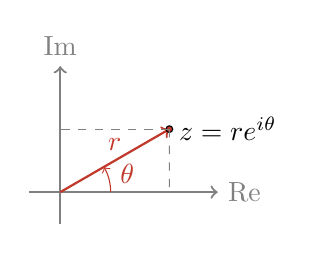
\begin{tikzpicture}[scale=0.8]
        % 坐标轴
        \draw[->, thick, gray] (-0.5,0) -- (2.5,0) node[right] {Re};
        \draw[->, thick, gray] (0,-0.5) -- (0,2.0) node[above] {Im};
        % 向量
        \draw[->, thick, section5] (0,0) -- (30:2) node[midway, above] {$r$};
        \draw[fill=section5] (30:2) circle (1.5pt) node[right] {$z=re^{i\theta}$};
        % 角度
        \draw[->, thin, section5] (0.8,0) arc (0:30:0.8);
        \node[section5] at (15:1.1) {$\theta$};
        % 辅助虚线
        \draw[dashed, gray] (30:2) -- (1.732,0);
        \draw[dashed, gray] (30:2) -- (0,1);
    \end{tikzpicture}
    \end{center}

\hspace{2em}如果说实数是一根直线,复数就是一个平面。引入复数不是为了把问题变复杂,而是为了利用二维空间的\textbf{对称性}来降维打击一维问题。
    \vspace{4pt}
    
    \subt{四大核心视角}
    \begin{itemize}[itemsep=4pt]
        \item \textbf{旋转即乘法}:
        $e^{i\theta}$ 是永不停歇的齿轮。所有波动本质上都是圆周运动的投影。
        
        \item \textbf{解析即全息 (Holographic)}:
        只要知道了一个小邻域的信息 (泰勒级数),理论上就能推导出整个定义域的函数值。\textbf{(解析延拓)}

        
        \item \textbf{物理的统一性}:
        量子力学的波函数、流体力学的势流、交流电的相量,底层共享同一套数学结构。
    \end{itemize}
    
    \vspace{6pt}
    \centering\textit{\footnotesize 现实世界是实数的,但理解它的钥匙往往是复数的。}
\end{mybox}

\end{multicols*}

\end{document}